\documentclass[11pt]{article}
\usepackage[margin=1.1in]{geometry}
\usepackage{graphicx}
\usepackage{booktabs}
\usepackage{amsmath}
\usepackage[round]{natbib}
\usepackage[hidelinks]{hyperref}
\usepackage{microtype}
\graphicspath{{../outputs/figures/}}

\title{When can you trust an ML streamflow forecast?\\
\large A California Sierra case study with Google's open flood-forecasting LSTM}
\author{Holden Leslie-Bole}
\date{2026-08-18 --- working draft for proofreading}

\newcommand{\finding}[1]{\section*{#1}}

\begin{document}
\maketitle

\begin{abstract}
\noindent Most machine-learning streamflow demonstrations end at a benchmark win. This
one starts at one --- the model does beat the process-model retrospective, on the window
where I first ran that comparison --- and then spends the rest of its effort finding out
where the win stops holding. It stops in five places, and the five boundaries turned out
to be more useful than the win. The model is a good 2-to-7-day volume forecaster for
gauged basins in a hydrologic regime it has seen. It is not a flood-peak predictor. At
one day ahead, outside rain-driven basins, it loses to yesterday's gauge reading. Held
out of its training set, it failed to transfer across a regime boundary. Its uncertainty
estimates are not yet calibrated. And its win over the process model depends on which
version of that model, and which years, you test against. Every one of those statements
is a measurement, not a hedge.
\end{abstract}

\section*{Setup}

\texttt{mean\_embedding\_forecast\_lstm}, hidden size 128, trained on 28 California
basins from the Caravan dataset \citep{kratzert2023caravan} with MultiMet forcing (HRES,
IMERG, CPC precipitation and temperature). I extended the streamflow targets from 2014 to
October 2024 using USGS NWIS so that two genuine flood water years could be held out.

\begin{figure}[htbp]
\centering
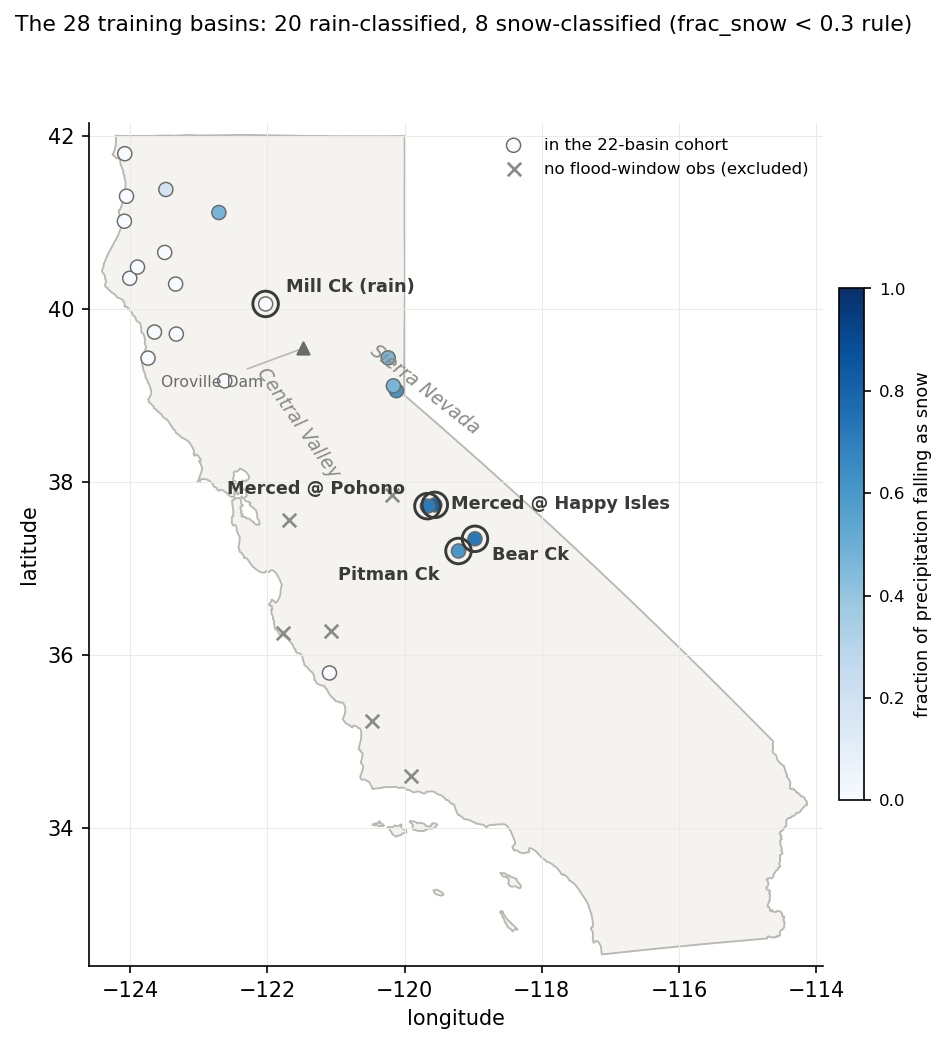
\includegraphics[width=0.78\textwidth]{study_map.png}
\caption{The 28 training basins. Color gives the fraction of precipitation falling as
snow (the regime variable behind Findings 1, 3 and 5); rings mark the five focus
basins; crosses mark the six basins with no flood-window observations, excluded from
every cohort median. The snowmelt focus basins sit in the high Sierra; Mill Creek, the
one rain-driven focus basin, drains the southern Cascades toward the Sacramento
Valley.}
\label{fig:map}
\end{figure}

\textbf{Test set: water years 2017 and 2023} --- the Oroville-spillway atmospheric-river
season and the 2023 AR sequence. Training uses every remaining day in the record outside
the test windows and the 2009--2011 validation years. Checkpoints are selected on
validation, not taken from the last epoch. Of the 28 trained basins
\citep[CAMELS;][]{newman2015camels}, 22 have observations in the flood windows (Figure~\ref{fig:map}); medians
below are over that fixed cohort, except the NWM comparison in Finding~5, which is over
the five focus basins where the NWM reaches were extracted.

The test-period choice is itself the first result. An earlier version of this work
tested on 2012--2014 and reported median NSE 0.81. That window is California drought
onset. Retrained and retested at the same capacity on the same 22 basins, the model
scores \textbf{0.862} on the drought window and \textbf{0.754} on the flood years
(0.836 and 0.679 at the smaller capacity) --- and the flood-year model sees eleven
\emph{more} years of training data, so if anything the gap is understated. The original
number wasn't wrong. It was measured on a benign period. Report streamflow skill without
saying which hydrologic years you tested on, and you're reporting the years, not the
model.

\finding{Finding 1 --- The baseline that matters is a gauge, not a mean}

NSE scores a forecast against the mean of the observations, which is a very weak null.
So I scored stronger ones on the identical test set and metric definitions, matched by
forecast lead --- a forecast for tomorrow and a forecast for next week are different
problems and deserve different nulls (Table~\ref{tab:persistence},
Figure~\ref{fig:crossover}).

\begin{table}[htbp]
\centering
\caption{Median NSE by forecast lead, flood-year test set. Damped persistence relaxes
the last gauge reading toward the day-of-year climatology at the training-fit
autocorrelation --- the standard stronger null. The train-period mean scores $-0.08$ and
raw climatology $+0.20$; neither is competitive. Bold marks the winner per cohort.}
\label{tab:persistence}
\begin{tabular}{lcccccc}
\toprule
 & \multicolumn{3}{c}{22-basin cohort} & \multicolumn{3}{c}{5 snowmelt focus basins} \\
\cmidrule(lr){2-4}\cmidrule(lr){5-7}
Lead (d) & LSTM & Persist. & Damped & LSTM & Persist. & Damped \\
\midrule
1 & 0.667 & 0.712 & \textbf{0.738} & 0.810 & 0.944 & \textbf{0.945} \\
2 & \textbf{0.688} & 0.484 & 0.566 & 0.810 & \textbf{0.864} & 0.869 \\
3 & \textbf{0.665} & 0.301 & 0.447 & 0.809 & 0.803 & \textbf{0.814} \\
5 & \textbf{0.670} & 0.037 & 0.340 & \textbf{0.802} & 0.702 & 0.725 \\
7 & \textbf{0.597} & $-0.122$ & 0.295 & \textbf{0.792} & 0.610 & 0.649 \\
\bottomrule
\end{tabular}
\end{table}

\begin{figure}[htbp]
\centering
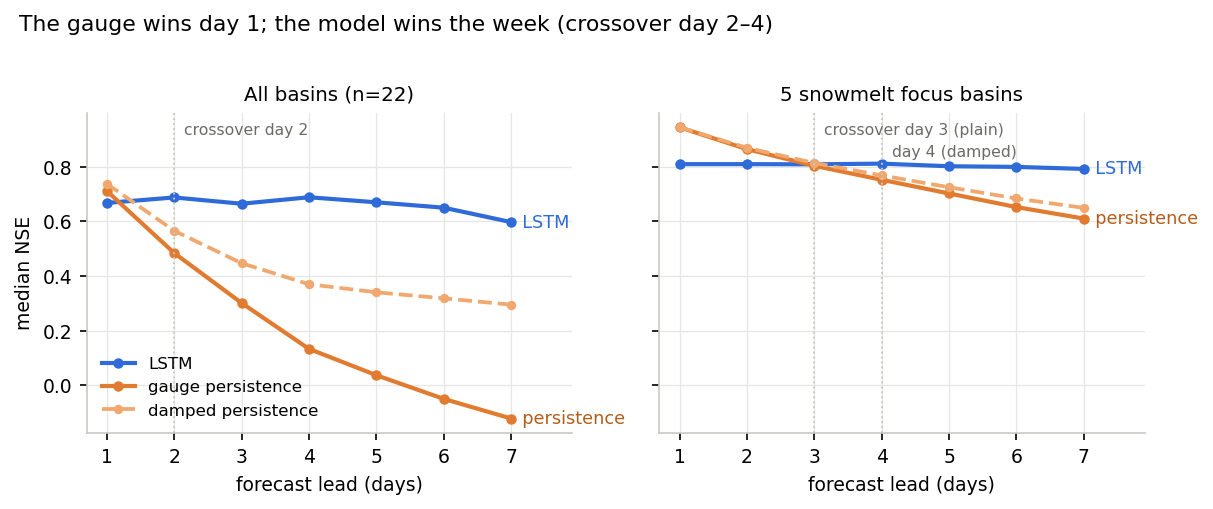
\includegraphics[width=\textwidth]{persistence_crossover.png}
\caption{Persistence decays with lead while the LSTM stays nearly flat; the model
overtakes at day 2 across the cohort and day 3--4 on the snowmelt focus basins.}
\label{fig:crossover}
\end{figure}

At one day ahead, the gauge beats the model nearly everywhere. Persistence decays with
lead; the LSTM barely does. The model pulls ahead at day 2 across the cohort, against
both nulls. On the high-storage snowmelt basins it takes until day 3 against plain
persistence and day 4 against the damped version. The one exception is the rain-driven
basin, where the LSTM wins at every lead (0.618 vs 0.594 damped at day 1) --- flashy
rain response just isn't persistent.

The information asymmetry here runs both ways, and both halves matter. The LSTM never
ingests observed discharge; persistence is built from a gauge reading the model is
denied, and a real flood operator has that gauge. But the LSTM ingests forecast
meteorology through the target day. It knows about the storm that hasn't arrived yet,
and persistence knows nothing about the future --- so at day 1 the model is losing to a
naive gauge reading \emph{despite} seeing tomorrow's precipitation. The next
architecture suggests itself: take both inputs, and assimilate the gauge.

One more note, on the climatology row: it scored $-0.25$ on the 2012--2014 drought
window and $+0.198$ on the flood years. A baseline's value is a property of the test
period, not of the baseline.

\finding{Finding 2 --- The model gets \emph{when}, not \emph{how big}}

On the held-out flood years the deterministic model posts NSE 0.754 and times peaks to
about a day. But its high-flow volume bias (FHV) is $-19\%$, it misses roughly 45\% of
peaks, and its peak magnitude error runs near 48\% (peak counts come from a few events
per basin over two water years, so treat those rows as coarse). Timing is good;
magnitude is not. For flood operations, where the decision is how much water to release
before a storm arrives, magnitude is the whole question
(Figure~\ref{fig:hydrographs}).

\begin{figure}[htbp]
\centering
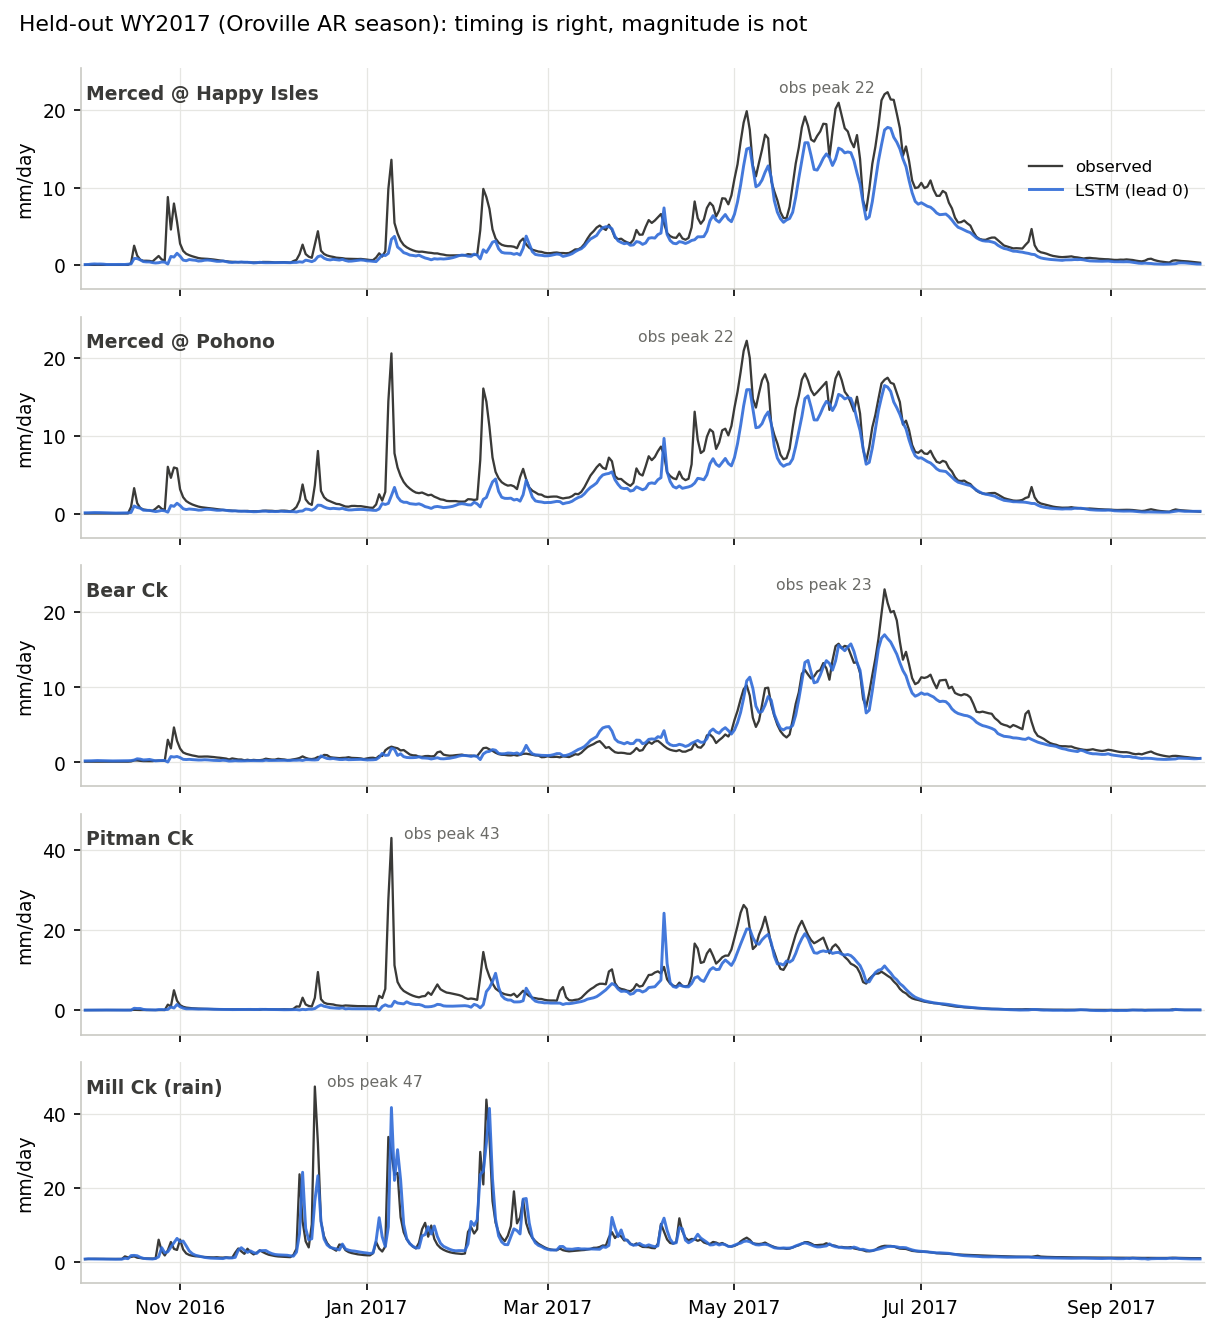
\includegraphics[width=\textwidth]{flood_hydrographs.png}
\caption{Held-out WY2017: the freshet and storm timing are captured; the snowmelt-basin
peaks come up short.}
\label{fig:hydrographs}
\end{figure}

This isn't an ML-specific failure. On a separately held-out extreme --- January 1997,
with the entire 1990s excluded from training --- both the LSTM and the NWM v2.1
retrospective underestimated the flood peak by tens of percent, and on the rain-driven
basin the process model caught the peak far better. (1997 predates the forecast-era
forcing products, so the LSTM also ran on degraded inputs there.) Underestimating flood
peaks is roughly the state of the art. Saying so is more useful than hiding it.

A capacity experiment sharpens the point. Raising hidden size from 16 to 128 improved
average skill (NSE $0.679 \rightarrow 0.754$) and made peaks worse: FHV slid from
$-12\%$ to $-19\%$, missed peaks from 0.33 to 0.45. More capacity bought accuracy on
the bulk of the distribution and paid for it in the tail, which is what regression
toward the mean on out-of-distribution extremes looks like --- though with one training
run per capacity, call it a consistent gradient rather than a seed-controlled
result.

\finding{Finding 3 --- It regionalizes within a regime and inverts across one}

Ungauged prediction is what water agencies actually need, because most basins have no
gauge. So I held each focus basin entirely out of training and asked the model to
predict it cold. Bear Ck (snowmelt) degraded to NSE 0.646 with $-29\%$ high-flow bias.
Pitman Ck (snowmelt) fell to 0.375 at $-62\%$. And Mill Ck --- the rain-driven basin ---
didn't degrade. It inverted: NSE $-0.740$, worse than predicting the mean, with the bias
flipping sign to $+80\%$ over-prediction (Figure~\ref{fig:lobo}).

\begin{figure}[htbp]
\centering
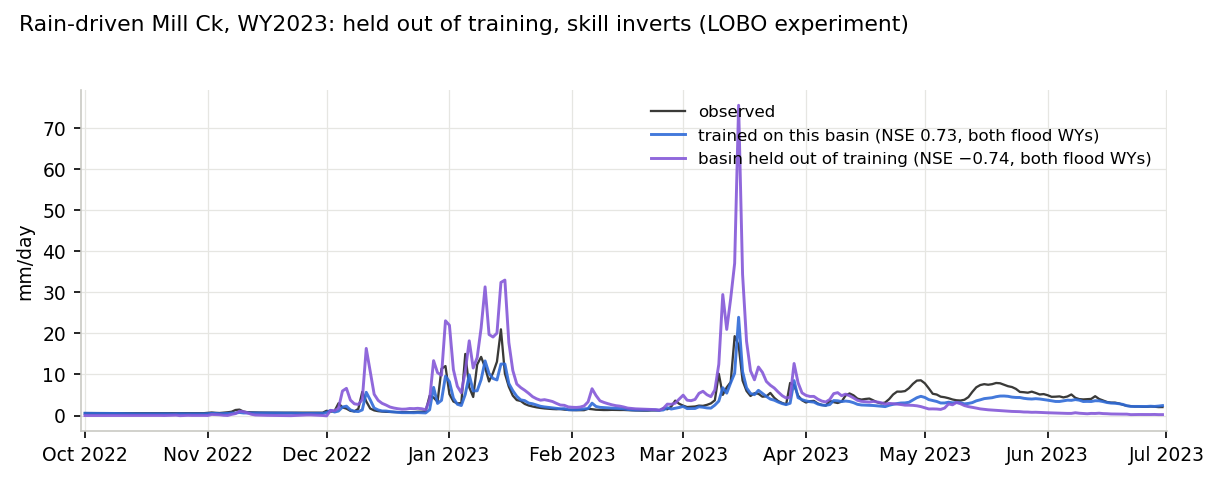
\includegraphics[width=\textwidth]{lobo_millck_inversion.png}
\caption{The same basin, two models: trained on it (blue) vs held out of training
(purple). The held-out model applies a snowmelt mapping to a rain basin and invents
peaks.}
\label{fig:lobo}
\end{figure}

Trained on 27 mostly-snowmelt catchments, the model learned snowmelt, and it
extrapolated snowmelt onto a rain-driven catchment it had never seen. This is one basin,
the only rain-driven one in the set --- a demonstration, not a statistic. It's also a
property of a small, regime-homogeneous training set: the regionalization successes in
the literature train on hundreds of hydrologically diverse basins
\citep{kratzert2019regional,nearing2024global}, and the diversity is the mechanism. The
fix is training-set diversity, not a different architecture. But the operational lesson
stands either way: a regional model will quietly extrapolate its regime onto basins that
don't share it. (Two further basins, the nested Merced pair, scored 0.857 and 0.790 ---
but each has its nested partner in the training set, which leaks the hydrograph, so I
exclude them from the ungauged claim.)

\finding{Finding 4 --- Sharper, and overconfident}

The framework can emit a full predictive distribution (a countable mixture of asymmetric
Laplacians) instead of a point estimate. Scored properly, this is where it gets
interesting.

CRPS generalizes MAE: for a point forecast, CRPS collapses exactly to the absolute
error, so both models can be scored on one proper rule \citep{gneiting2007strictly}
with no special-casing, using the fair (finite-ensemble-unbiased) estimator
\citep{ferro2014fair} --- and the ensemble only wins if its spread carries real
information. It does. CRPS (in mm/day) drops from 1.231 to 0.916 at the same-day
nowcast, 1.452 to 1.081 at three days, 1.550 to 1.185 at seven --- a 22--26\%
improvement at every lead. The distributional head also edges the deterministic model on
point metrics (NSE 0.784 vs 0.754, fewer missed peaks, smaller peak error, at some cost
in KGE). An earlier draft called the two models tied; that reading traced back to a
scoring-pipeline bug, not to the models.

But the intervals are not calibrated. A nominal 90\% predictive interval covers 66--74\%
of observations. The forecast is better \emph{and} overconfident about being better,
which for an operator is the dangerous direction (Figure~\ref{fig:calibration}).

\begin{figure}[htbp]
\centering
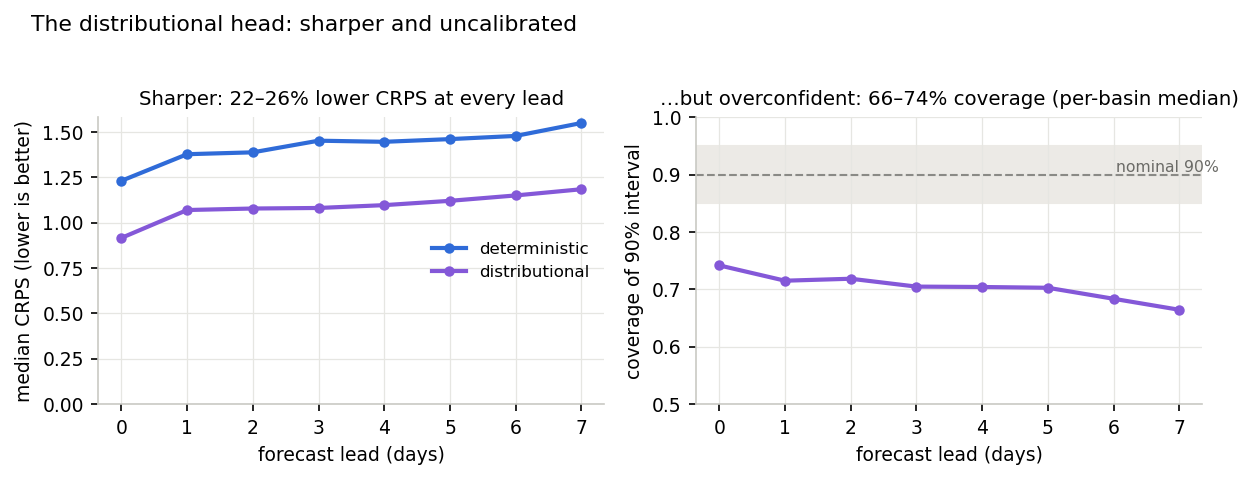
\includegraphics[width=\textwidth]{crps_calibration.png}
\caption{Sharper on CRPS at every lead, yet the nominal 90\% interval covers only
66--74\% of observations.}
\label{fig:calibration}
\end{figure}

The rank histogram says why, and it isn't the obvious story (Figure~\ref{fig:pit}). In
aggregate the histogram is U-shaped and nearly symmetric --- 22\% of observations land
above the ensemble's 90th percentile rank, 20\% below the 10th --- which reads as simple
under-dispersion. Condition on flow, though, and the misses split with opposite signs:
at high flows the observation escapes above the interval (23\% above vs 3\% below), and
at low flows it escapes below (23\% vs 9\%). The predictive distribution isn't merely
too narrow. It's pulled toward the middle of the flow distribution at both ends ---
regression toward the mean again, this time expressed distributionally. (A separate and
genuine heavy-tail pathology, rare extreme samples that inflate the ensemble standard
deviation to about three times the RMSE, explains the spread/skill paradox and the NaN
training losses. It does not explain the coverage failure.)

\begin{figure}[htbp]
\centering
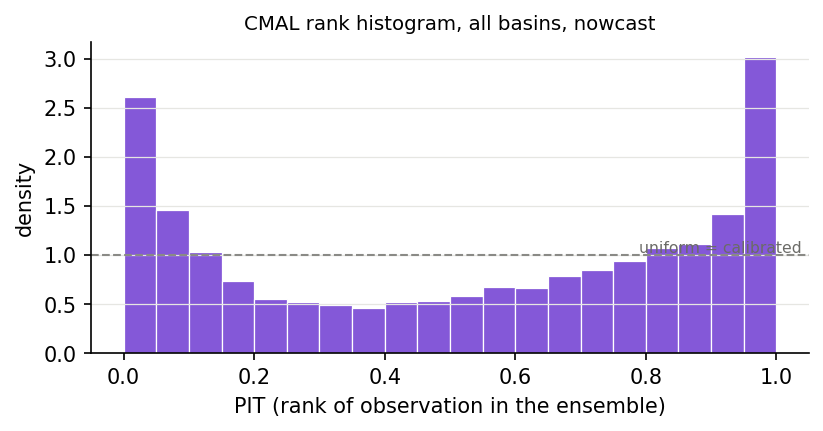
\includegraphics[width=0.62\textwidth]{pit_histogram.png}
\caption{The rank histogram: U-shaped in aggregate, but the two tails come from
different flows --- high flows escape above the interval, low flows below.}
\label{fig:pit}
\end{figure}

That diagnosis constrains the remedy. Uniform variance inflation would widen intervals
everywhere and still miss high-flow observations sitting above a displaced center. The
fix has to be flow-conditional --- recalibration by flow band, or a bias-aware head ---
and whatever fixes coverage has to be checked against the 22--26\% CRPS gain it could
erode.

\finding{Finding 5 --- The benchmark win depends on the benchmark}

The result this project once led with: on the 2012--2014 window, the LSTM beat the NOAA
National Water Model v2.1 retrospective on every focus basin, median NSE 0.83 vs 0.53.
Rerun on the flood years, against both v2.1 and the current v3.0, that headline does not
survive intact (Table~\ref{tab:nwm}, Figure~\ref{fig:nwm}).

\begin{table}[htbp]
\centering
\caption{Focus-basin medians, flood windows. The v3.0 retrospective ends 2023-02-01, so
the WY2023 window is October--January: it covers the December--January AR sequence but
not the March storms.}
\label{tab:nwm}
\begin{tabular}{lccc}
\toprule
Window & LSTM & NWM v2.1 & NWM v3.0 \\
\midrule
WY2017, median NSE & 0.772 & 0.628 & \textbf{0.848} \\
WY2017, high-flow bias & $-20\%$ & $-2\%$ & $\mathbf{-5\%}$ \\
WY2023 (Oct--Jan), median NSE & \textbf{0.443} & --- & 0.162 \\
\bottomrule
\end{tabular}
\end{table}

\begin{figure}[htbp]
\centering
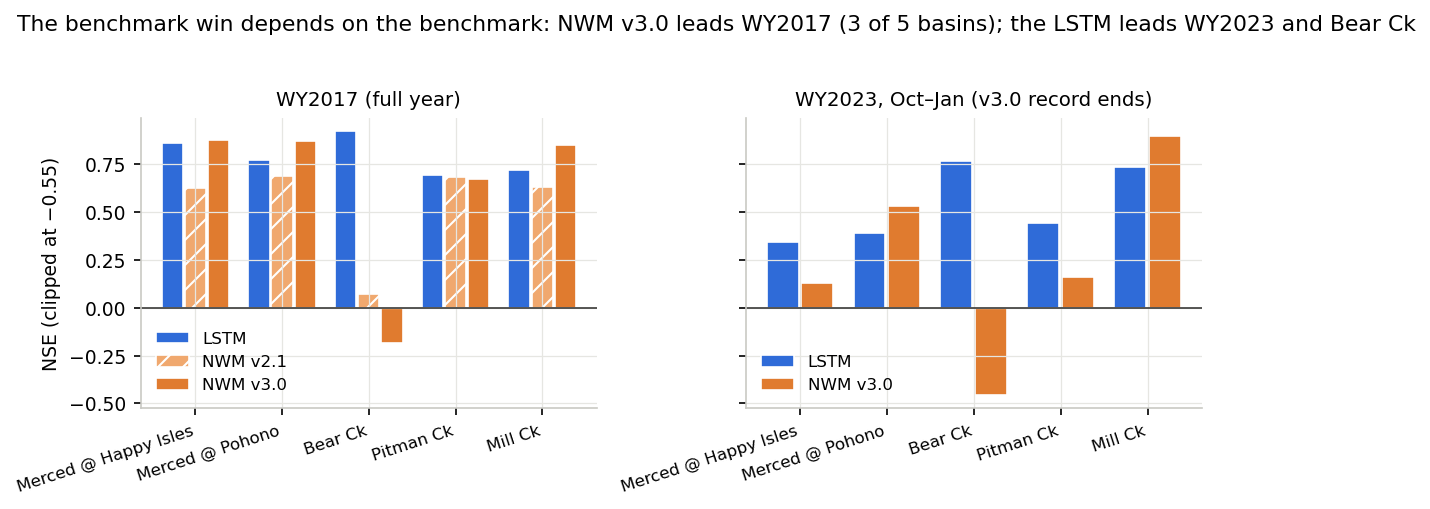
\includegraphics[width=\textwidth]{lstm_vs_nwm_flood.png}
\caption{Per-basin NSE on the flood windows. The NWM v3.0 retrospective leads WY2017 on
three of five basins (not Bear Ck or Pitman Ck); the LSTM leads the WY2023 window except
at rain-driven Mill Ck.}
\label{fig:nwm}
\end{figure}

A protocol note first: these are the NWM \emph{retrospectives} --- analysis-forced,
open-loop simulations --- against the LSTM's same-day hindcast. It's a
simulation-vs-simulation comparison, not operational forecast skill, and the operational
NWM additionally assimilates gauges. With that said: on WY2017 the modern NWM beats the
LSTM on median skill, winning three of five basins, and is far better on high-flow bias
and peak error. A large share of the original margin was the NWM \emph{version}, not
the physics. On the partial WY2023 window the LSTM wins on median skill --- and both
systems underestimate high flows by around 53--55\%.

Two structural results are stable in every window I tested. The LSTM wins Bear Creek
decisively in both flood years (0.92 and 0.77, against at best 0.07) --- a
high-elevation, high-storage snowmelt basin where the NWM's snow physics reliably
fails. And the process model wins rain-driven flood peaks (Mill Creek: 0.90 vs 0.74 in
WY2023, with the same signature in 1997), because explicit routing captures what
regression toward the mean smooths away.

``ML beats the operational model'' turns out not to be a finding. It's a claim indexed
by model version, test years, and hydrologic regime. The finding that survives is the
complementarity: each model dominates where the other's structure fails.

\finding{The winter everyone is watching}

As I write this (August 2026), NOAA's Climate Prediction Center has El Ni\~no conditions
in place with better than 90\% odds of a very strong event this winter and roughly 60\%
odds it peaks at ``super'' magnitude \citep{cpc2026enso} --- and the press has spent the
summer asking whether 2026--27 could be the winter California draws an ARkStorm-class
sequence, the parade-of-ARs megaflood scenario the USGS first gamed out
\citep{porter2011arkstorm} and \citet{huang2022climate} updated. My Scripps colleagues
at CW3E published the sober version of the outlook this year
\citep{gershunov2025atmospheric}: in California's changing hydroclimate, precipitation
events of the 1997 New Year's flood class --- the same 1997 event held out in
Finding~2 --- are headed toward twice their historical likelihood by late century. So
it's fair to ask what this evaluation implies about leaning on a model like this one in
a winter like that.

Two honest caveats before the implications. ENSO loads the dice; it doesn't roll them
--- the wettest year in this record, WY2023, arrived during La Ni\~na. And what a strong
El Ni\~no most reliably changes is storm \emph{character}: a southward-shifted
subtropical jet and warmer atmospheric rivers with high snow levels, which is to say
more rain falling on basins that usually take snow.

Read against that scenario, the five findings stop being abstract:

\begin{itemize}
\item \textbf{The peaks would be missed low.} Every model tested here underestimates
flood-peak magnitude on out-of-distribution extremes, the LSTM by 40--80\% on
1997-class events --- and the capacity experiment suggests bigger networks regress
harder. An ARkStorm-class sequence sits farther outside the training distribution than
anything I could test: the largest events in this model's 40-year training record are
precisely the WY2017 and WY2023 storms it under-predicted by half.
\item \textbf{Warm ARs push basins across the regime boundary this model fails at.}
High snow levels turn snowmelt catchments into temporary rain catchments --- the
direction of the Mill Creek inversion, and the place where the NWM's explicit routing
beat the LSTM on peaks in both 1997 and 2023. In exactly the scenario people are
worried about, the complementarity argument becomes operational advice: run both model
families, and weight the process model's peaks.
\item \textbf{The uncertainty estimates fail worst where that winter would live.} The
distributional head's intervals are overconfident specifically at high flows ---
observations escape above the interval seven times more often than below. Until
calibration is fixed flow-conditionally, the intervals should not be trusted in an AR
sequence, full stop.
\item \textbf{The value that survives is the 2-to-7-day window.} That happens to be the
lead time that matters for pre-storm reservoir releases --- the FIRO
(forecast-informed reservoir operations) window CW3E has been building toward for a
decade --- and it's where this model class genuinely beats both persistence and, on
storage-dominated basins, the NWM. It's also the window where skill inherits directly
from the forcing, so every improvement AR Reconnaissance buys in landfall forecasts
flows straight through a forcing-driven model like this one.
\end{itemize}

There's also a concrete experiment sitting here that I haven't run: ARkStorm~2.0 exists
as simulated meteorology \citep{huang2022climate}. Feeding that forcing through this
trained model would measure directly how a data-driven forecaster degrades on an event
beyond its training distribution --- before the atmosphere runs the experiment for us.

\finding{What this adds up to}

\begin{table}[htbp]
\centering
\caption{Verdicts by use case.}
\label{tab:verdict}
\begin{tabular}{p{0.42\textwidth}p{0.5\textwidth}}
\toprule
Use case & Verdict \\
\midrule
2--7 day volume forecast, gauged basin, regime seen in training & \textbf{Yes} --- beats persistence (plain and damped) from day 2--4 and holds skill where both collapse \\
1-day forecast & \textbf{No} on snowmelt/high-storage basins --- the gauge is better, and free; on rain-driven basins the LSTM already wins at day 1 \\
Flood peak magnitude & \textbf{Not yet} --- and the process model largely shares the failure \\
Ungauged basin in an unseen regime & \textbf{No} --- skill inverts \\
Calibrated uncertainty & \textbf{Not yet} --- but most fixable, and the sharpness gain (22--26\% CRPS) is real \\
Replacing the process model & \textbf{No} --- the v3.0 retrospective wins WY2017 on 3 of 5 basins; the models are complementary by regime \\
\bottomrule
\end{tabular}
\end{table}

The strongest claim this work supports is not ``ML beats the operational model.'' It's
narrower and more useful: ML delivers real, measurable forecast value in gauged,
in-regime basins at 2-to-7-day leads, and the boundaries of that value are measurable
--- in five independent ways.

\finding{Reproducibility}

Every number above comes from a single scoring protocol: simulations read from each
run's inference output, observations taken from the source gauge records (never from a
model run's own copy), the framework's metric implementations, checkpoints chosen on
validation, and a stated 22-basin cohort. Deterministic inference reproduced
bit-for-bit across repeated runs. The distributional model's sample-median metrics carry
a bootstrap uncertainty below 0.001 NSE, so reported differences are not
ensemble-sampling noise --- though each configuration is a single training run, and
seed-to-seed variance is the axis I haven't controlled.

The protocol looks the way it does because closure tests kept catching real problems: a
test-period choice that flattered skill by 0.11 NSE, an evaluation code path that
silently dropped over a quarter of the scoreable basins from its medians, and an
upstream bug that writes corrupted observations into the distributional model's output
files --- caught because two metrics that could not both be true showed up together, and
the observations, not the model, turned out to be the thing to check. The record
extension was validated by closure against the overlapping original record, which
surfaced a per-basin catchment-area discrepancy and five gauges whose records genuinely
disagree; I excluded those rather than silently rescaling them.

Known limitations, failure modes, and the traps encountered along the way are documented
in \texttt{docs/METHODS.md} in the project repository:\\
\url{https://github.com/holdenlesliebole/central-valley-flood-lstm}.

\bibliographystyle{plainnat}
\bibliography{refs}

\end{document}
